\documentclass[handout]{beamer}\usepackage[]{graphicx}\usepackage[]{color}
%% maxwidth is the original width if it is less than linewidth
%% otherwise use linewidth (to make sure the graphics do not exceed the margin)
\makeatletter
\def\maxwidth{ %
  \ifdim\Gin@nat@width>\linewidth
    \linewidth
  \else
    \Gin@nat@width
  \fi
}
\makeatother

\definecolor{fgcolor}{rgb}{0.345, 0.345, 0.345}
\newcommand{\hlnum}[1]{\textcolor[rgb]{0.686,0.059,0.569}{#1}}%
\newcommand{\hlstr}[1]{\textcolor[rgb]{0.192,0.494,0.8}{#1}}%
\newcommand{\hlcom}[1]{\textcolor[rgb]{0.678,0.584,0.686}{\textit{#1}}}%
\newcommand{\hlopt}[1]{\textcolor[rgb]{0,0,0}{#1}}%
\newcommand{\hlstd}[1]{\textcolor[rgb]{0.345,0.345,0.345}{#1}}%
\newcommand{\hlkwa}[1]{\textcolor[rgb]{0.161,0.373,0.58}{\textbf{#1}}}%
\newcommand{\hlkwb}[1]{\textcolor[rgb]{0.69,0.353,0.396}{#1}}%
\newcommand{\hlkwc}[1]{\textcolor[rgb]{0.333,0.667,0.333}{#1}}%
\newcommand{\hlkwd}[1]{\textcolor[rgb]{0.737,0.353,0.396}{\textbf{#1}}}%

\usepackage{framed}
\makeatletter
\newenvironment{kframe}{%
 \def\at@end@of@kframe{}%
 \ifinner\ifhmode%
  \def\at@end@of@kframe{\end{minipage}}%
  \begin{minipage}{\columnwidth}%
 \fi\fi%
 \def\FrameCommand##1{\hskip\@totalleftmargin \hskip-\fboxsep
 \colorbox{shadecolor}{##1}\hskip-\fboxsep
     % There is no \\@totalrightmargin, so:
     \hskip-\linewidth \hskip-\@totalleftmargin \hskip\columnwidth}%
 \MakeFramed {\advance\hsize-\width
   \@totalleftmargin\z@ \linewidth\hsize
   \@setminipage}}%
 {\par\unskip\endMakeFramed%
 \at@end@of@kframe}
\makeatother

\definecolor{shadecolor}{rgb}{.97, .97, .97}
\definecolor{messagecolor}{rgb}{0, 0, 0}
\definecolor{warningcolor}{rgb}{1, 0, 1}
\definecolor{errorcolor}{rgb}{1, 0, 0}
\newenvironment{knitrout}{}{} % an empty environment to be redefined in TeX

\usepackage{alltt}

\usetheme{AnnArbor}
\usecolortheme{beaver}

\usepackage[font=footnotesize,labelfont=bf]{caption}


\setlength{\unitlength}{\textwidth}  % measure in textwidths
\usepackage[normalem]{ulem}
\usepackage{multicol}

\setbeamertemplate{navigation symbols}{}
\setbeamertemplate{enumerate items}[default]
\setbeamertemplate{enumerate subitem}{\alph{enumii}.}
\setbeamertemplate{enumerate subsubitem}{\roman{enumiii}.}
\setkeys{Gin}{width=0.6\textwidth}

\title{Measuring Energy Intake via Energy Balance Principle While Accounting for Measurement Error}
\author[Danny Ries]{Danny Ries}
\institute[Iowa State]{Iowa State University}
\date{June 22, 2016}

\newcommand{\mG}{\mathrm{\Gamma}}
\newcommand{\I}{\mathrm{I}}
\newcommand{\mySigma}{\mathrm{\Sigma}}
\newcommand{\ind}{\stackrel{ind}{\sim}}
\IfFileExists{upquote.sty}{\usepackage{upquote}}{}
\begin{document}

%\section{Temp??} \begin{comment}







\frame{\maketitle}

\section{Introduction}
\subsection{Motivation}
%--------
\begin{frame}
\frametitle{The Obesity Epidemic}

Over 35\% of Americans are obese, and over  75\% of men are either overweight or obese. Obesity is linked to many different medical, psychological, emotional, and economic effects such as:
\begin{itemize}
\begin{multicols}{2}
\item
Type 2 Diabetes
\item
Coronary Heart Disease
\item
High Blood Pressure
\item 
Clinical Depression
\columnbreak
\item
Anxiety
\item 
Increased Health Care Costs
\item
Lost Wages
\item
Discrimination
\end{multicols}
\end{itemize}

\end{frame}

%-----------



\subsection{Fatal Flaw}

%----------
\begin{frame}
\frametitle{The ``Fatal Flaw in Obesity Research"}
It has been said the ``Fatal Flaw in Obesity Research" is our inability to accurately measure how much someone eats (EI) in free living situations

\begin{itemize}
\item
Current measures of EI; ie. self report, are clouded with (measurement) error \\
\item
Garbage in Garbage out \\
\item
Tough to understand dietary trends over the years \\
\item
Cannot measure adherence to clinically prescribed interventions \\
\end{itemize}

This error in measurement extends to EE and body composition, albeit not nearly as severe

\end{frame}

%---------------

%-----------
\begin{frame}
\frametitle{2 Remedies to aid in Obesity Research}
\begin{enumerate}
\item
Accurately and efficiently measure Energy Intake (EI)

\vspace{0.2cm}

\item
Assess compliance to \emph{2008 Physical Activity Guidelines}
\end{enumerate}

%\vspace{0.2cm}

%A common issue here is we are dealing with 

\end{frame}
%-----------

\subsection{}

%-----------
\begin{frame}
\frametitle{Modeling Energy Balance}

\begin{block}{Energy Balance}
The application of the first law of thermodynamics to nutrition/exercise science: \\
Change in Energy Stores ($\Delta$ES) = Energy Intake (EI) - Energy Expenditure (EE)
\end{block}

where $\Delta$ES $= c_1 \frac{\Delta FM}{\Delta T } + c_2 \frac{\Delta FFM}{\Delta T}$  

\vspace{0.4cm}

This provides an alternative way to measure EI for an individual


\end{frame}
%-----------

%-----------
\begin{frame}
\frametitle{Modeling Energy Balance Cont.}
We are now in a situation where we must measure both EE and $\Delta$ES in order to calculate EI \\
$\rightarrow$ But gold standard measures for both exist!

\vspace{0.3cm}

In a world of unlimited resources, researchers needing EI for individuals could use gold standard measures of EE and $\Delta$ES and use simple measurement error models\\

\vspace{0.3cm}

Unfortunately,\\
DLW $\sim$ \$500/person \\
DXA $\sim$ \$100/person

\end{frame}
%----------

%----------
\begin{frame}
\frametitle{Modeling Energy Balance Cont.}
There are many other cheaper measures of EE and $\Delta$ES, that even when used together to calculate EI, are still more accurate than self-reported EI \\

\vspace{0.4cm}

Goal: Create a statistical measurement model for gold standard and cheap measurements of both EE and $\Delta$ES in order to develop calibration equations for cheap measurements.\\

\vspace{0.4cm}

This will allow future research to calibrate cheaper measurements (when gold standard measures aren't used) and thus eliminate known biases

\end{frame}
%----------

%----------
\begin{frame}
\frametitle{Modeling Energy Balance Cont. }

\begin{itemize}
\item
Lots of research has been done for calibrating and evaluating measurement error for EI
\item
Some research for EE
\item
Little research for $\Delta$ES
\end{itemize}

\vspace{0.2cm}

To the best of our knowledge, no research has been done in evaluating the measurement error and calibrating measurements jointly via the Energy Balance principle


\end{frame}
%----------


%---------
\begin{frame}
\frametitle{Energy Balance Study}
The Energy Balance Study (EBS) was conducted 2011-2012 at the University of South Carolina
\begin{itemize}
\item
430 male and females aged 20-35 \\
\item
5 DXA scans, one every 3 months
\item
Sensewear Armband measuring EE every 3 months (averaged across 10 days)
\item
Subset of 119 participants receieved DLW at end of 12 months, with additional DXA scan
\item
Demographic variables
\end{itemize}

\vspace{0.2cm}

Although these data don't have perfect replicates, it provides a baseline to start our modeling of measurement error in Energy Balance


\end{frame}
%--------

%--------
\begin{frame}
\frametitle{Checking Normality of Measurement Errors}

\begin{figure}
\centering
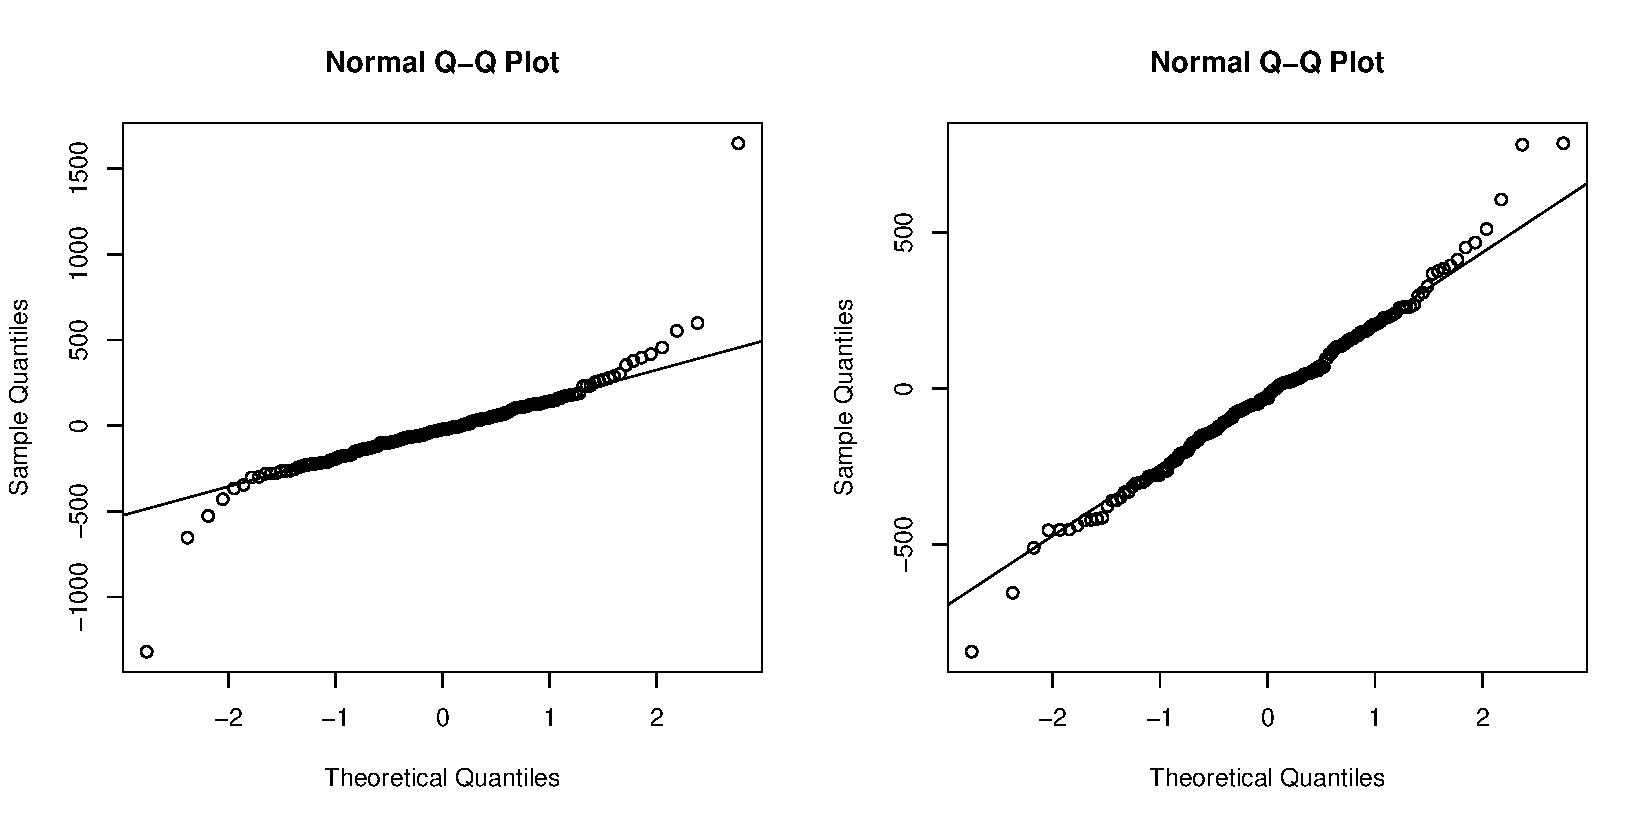
\includegraphics[width=10cm,height=5cm]{dxa_qq.pdf}
\caption{\small{Differenced DXA $\Delta$ES }}
\end{figure}

\end{frame}
%---------

%---------
\begin{frame}
\frametitle{Checking Normality of Measurement Errors}


\begin{figure}
\centering
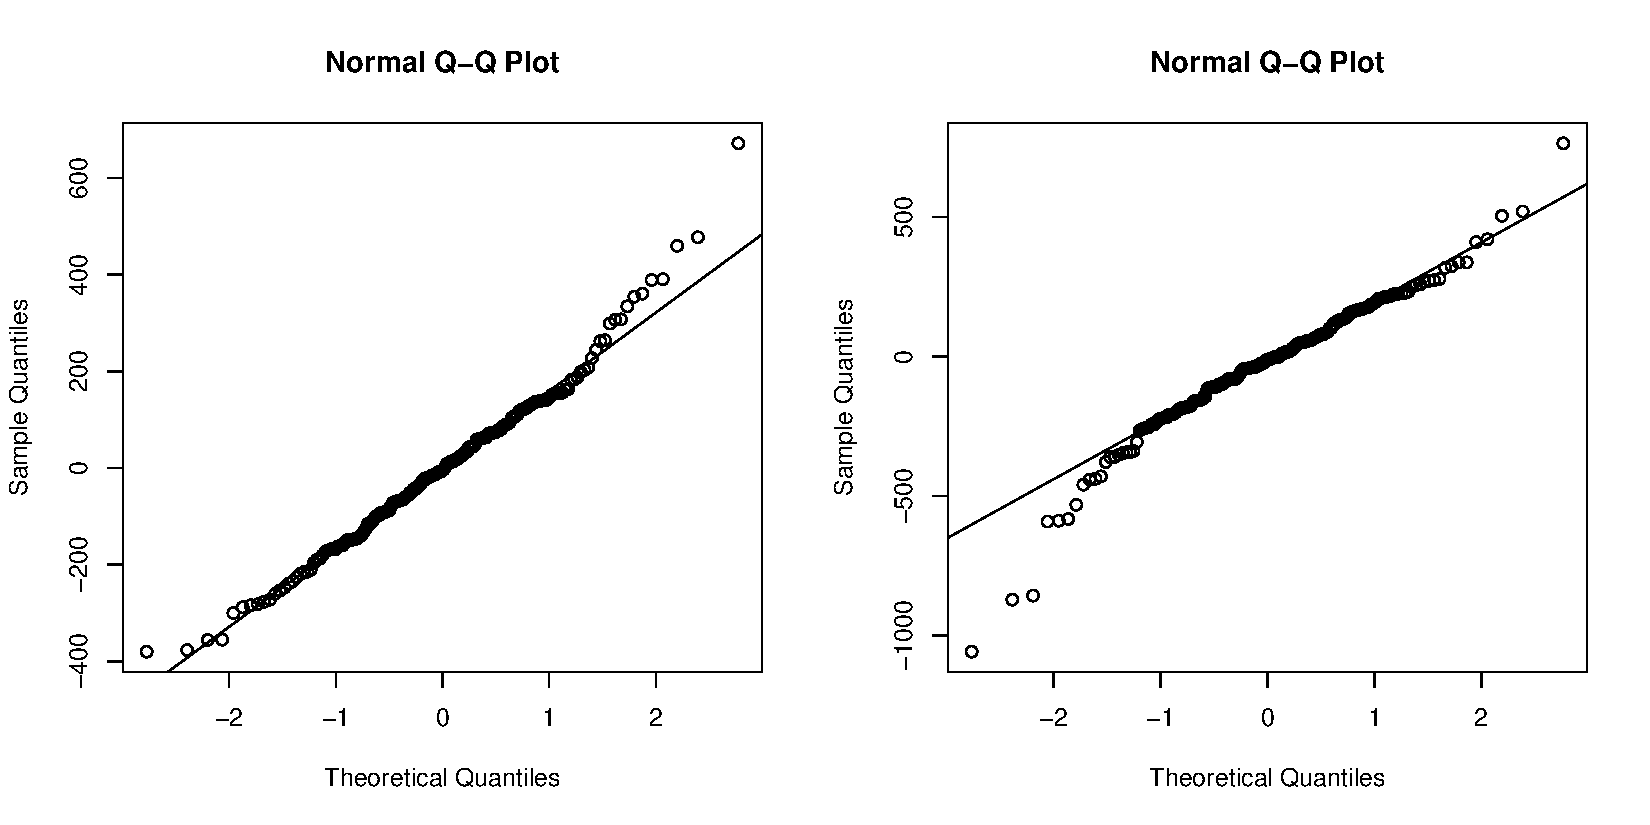
\includegraphics[width=10cm,height=5cm]{swa_qq.pdf}
\caption{Differenced SWA  EE }
\end{figure}


\end{frame}
%--------

%--------
\begin{frame}
\frametitle{N{\"a}ive Check for Biases}
It seems reasonable that cheap measurement tools could be affected by factors other than the \emph{truth}, ie. demographics \\

\vspace{0.3cm}

$\rightarrow$ Fit the following multiple regression model with the subset data from EBS\\
SWA EE = $\beta_0 + \beta_1$DLW EE + $\beta_z$' Demographic Variables + $\epsilon$ \\

\vspace{0.3cm}

This is not ideal since we would want True EE not DLW EE in the regression, but still provides motivation


\end{frame}
%-------

%-------
\begin{frame}

\begin{table} \centering 
  \caption{Regression of Sensewear Armband EE on DLW EE, Age, BMI, Gender using EBS data. Results show systematic biases could exist in cheap EE measurements.} 
\begin{tabular}{l|ccc}
\hline
Coefficient & Estimate & Std Error & P-value \\
\hline
Intercept & 878.422 & 154.113 & $<$0.0001 \\
DLW EE & 0.558 & 0.040 & $<$0.0001 \\
Age & -7.351 & 3.999 & 0.0676 \\
Male & 305.582 & 43.258 & $<$0.0001 \\
BMI & 14.146 & 3.988 & 0.0004 \\
\hline
\end{tabular} 
\end{table} 
\end{frame}
%-------


%-------
\begin{frame}
\frametitle{Notation}
let $i$ represent individual and $j$ represent replicate number \\

\vspace{0.3cm}

Observable:
\begin{itemize}
\item
$W_{ij}^{EE}$ and $W_{ij}^{\Delta ES}$ represent gold standard measures of EE and $\Delta$ES
\item
$Y_{ij}^{EE}$ and $Y_{ij}^{\Delta ES}$ represent cheap measures of EE and $\Delta$ES
\item
$Z_i$ represent a $k\times 1$ vector of error free covariates
\end{itemize}

\vspace{0.2cm}

Latent:
\begin{itemize}
\item
$X_{i}^{EE}$ and $X_{i}^{\Delta ES}$ represent \emph{usual} EE and $\Delta$ES

\end{itemize}

\end{frame}
%-------


%-------
\begin{frame}
\frametitle{Independence Assumptions}
Given $X_i^{EE}, Z_i$

\begin{itemize}
\item
$Y^{EE}_{ij}$ are mutually independent for all $i,j$ \\
\item
$W_{ij}^{EE}$ are mutually independent for all $i,j$ \\
\item
$Y_{ij}^{EE}$ is independent of $W_{ij}^{EE}$ for all $i,j$ \\
\item
$Y_{ij}^{EE}$ is independent of $W_{ij}^{\Delta ES}$ and $Y_{ij}^{\Delta ES}$ for all $i,j$ \\
\item
$W_{ij}^{EE}$ is independent of $W_{ij}^{\Delta ES}$ and $Y_{ij}^{\Delta ES}$ for all $i,j$ \\
\end{itemize}

\vspace{0.2cm}

Same assumptions hold for reverse case (replace EE with $\Delta$ES and $\Delta$ES with EE)


\end{frame}
%-------


%-------
\begin{frame}
\frametitle{Model for Observed Variables}


\begin{align*}
  Y_{ij}^{EE} &= m_{ee}(X_i^{EE} ,Z_i) + \epsilon_{ij}^{EE}   \\
   %& \\
  %
  Y_{ij}^{\Delta ES} &= m_{es}(X_i^{\Delta ES} ,Z_i) + \epsilon_{ij}^{\Delta ES} \\
  %
     %& \\
  W_{ij}^{EE} &= X_i^{EE}  + \nu_{ij}^{EE} \\
  %
     %& \\
  W_{ij}^{\Delta ES} &= X_i^{\Delta ES}  + \nu_{ij}^{\Delta ES}
\end{align*}

\vspace{0.5cm}
$E(\epsilon_{ij}^{EE}) = E(\epsilon_{ij}^{\Delta ES}) = E(\nu_{ij}^{EE}) = E(\nu_{ij}^{\Delta ES}) = 0$

\end{frame}
%------

%----------------
\begin{frame}
\frametitle{Joint Likelihood}
%Using conditional independence assumptions, our joint probability model for our observed data can be represented by:

\scalebox{0.67}{\parbox{.5\linewidth}{%
\begin{align*}
  \begin{split}
      \label{truedist}
  L_i(\boldsymbol{\theta}) &= \prod_{j=1}^{J} f(W_{ij}^{EE},W_{ij}^{\Delta ES}, Y_{ij}^{EE},Y_{ij}^{\Delta ES}|Z_i,\boldsymbol{\theta})  \\
   &=  \int_{\mathcal{X}_{es}} \int_{\mathcal{X}_{ee}} \prod_{j=1}^{J} f({ W_{ij}^{EE},W_{ij}^{\Delta ES}, Y_{ij}^{EE},Y_{ij}^{\Delta ES}, X_i^{EE}, X_i^{\Delta ES}|Z_i},\boldsymbol{\theta}) d{ X_i^{EE}} d{ X_i^{\Delta ES}} \\
  %
    &= \prod_{j=1}^{J} \int_{\mathcal{X}_{es}} \int_{\mathcal{X}_{ee}} f({ W_{ij}^{EE}|X_i^{EE},X_i^{\Delta ES},Z_i},\boldsymbol{\theta_{wee}}) f({ W_{ij}^{\Delta ES}|X_i^{EE},X_i^{\Delta ES},Z_i},\boldsymbol{\theta_{wes}}) \times\\
  & f({ Y_{ij}^{EE}|X_i^{EE},X_i^{\Delta ES},Z_i},\boldsymbol{\theta_{yee}}) f({ Y_{ij}^{\Delta ES}|X_i^{EE},X_i^{\Delta ES},Z_i},\boldsymbol{\theta_{yes}})  
   f({ X_i^{EE}, X_i^{\Delta ES}|Z_i},\boldsymbol{\theta_x}) d{ X_i^{EE}} d{ X_i^{\Delta ES}} \\
  %
  &= \prod_{j=1}^{J} \int_{\mathcal{X}_{es}} \int_{\mathcal{X}_{ee}} f({ W_{ij}^{EE}|X_i^{EE},Z_i},\boldsymbol{\theta_{wee}}) f({ W_{ij}^{\Delta ES}|X_i^{\Delta ES},Z_i},\boldsymbol{\theta_{wes}}) \times\\
  & f({ Y_{ij}^{EE}|X_i^{EE},Z_i},\boldsymbol{\theta_{yee}}) f({ Y_{ij}^{\Delta ES}|X_i^{\Delta ES},Z_i},\boldsymbol{\theta_{yes}})  
   f({ X_i^{EE}, X_i^{\Delta ES}|Z_i},\boldsymbol{\theta_x}) d{ X_i^{EE}} d{ X_i^{\Delta ES}} 
  \end{split}
  & \\
  & \\
  L(\boldsymbol{\theta}) &= \prod_{i=1}^{n}  L_i(\boldsymbol{\theta}) 
\end{align*}
}}



\end{frame}

%-------------

%-------
\begin{frame}
\frametitle{We can create energy!}

\begin{multicols}{2}
\begin{knitrout}\tiny
\definecolor{shadecolor}{rgb}{0.969, 0.969, 0.969}\color{fgcolor}

{\centering 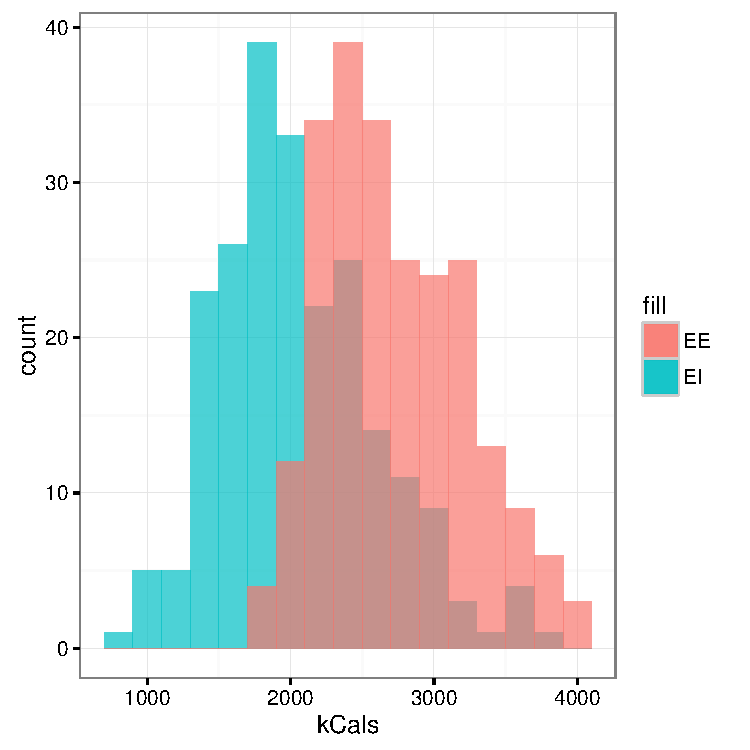
\includegraphics[width=.8\linewidth]{figure/eivsee-1} 

}



\end{knitrout}

\columnbreak
\pause
\begin{knitrout}\tiny
\definecolor{shadecolor}{rgb}{0.969, 0.969, 0.969}\color{fgcolor}

{\centering 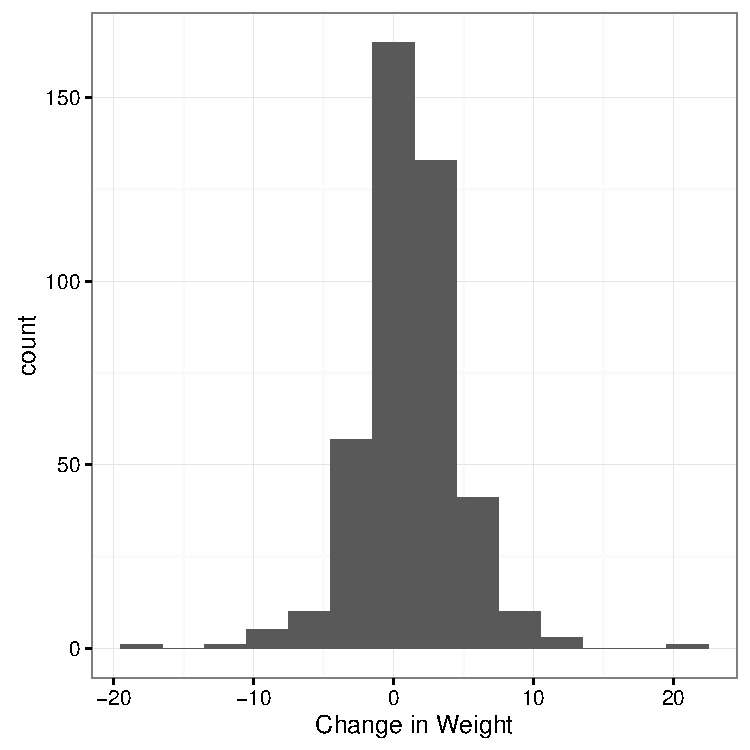
\includegraphics[width=.8\linewidth]{figure/eivsee2-1} 

}



\end{knitrout}

\end{multicols}

*Data from Energy Balance Study

\end{frame}

\begin{frame}
\frametitle{Armband vs DLW}
\begin{knitrout}\tiny
\definecolor{shadecolor}{rgb}{0.969, 0.969, 0.969}\color{fgcolor}

{\centering 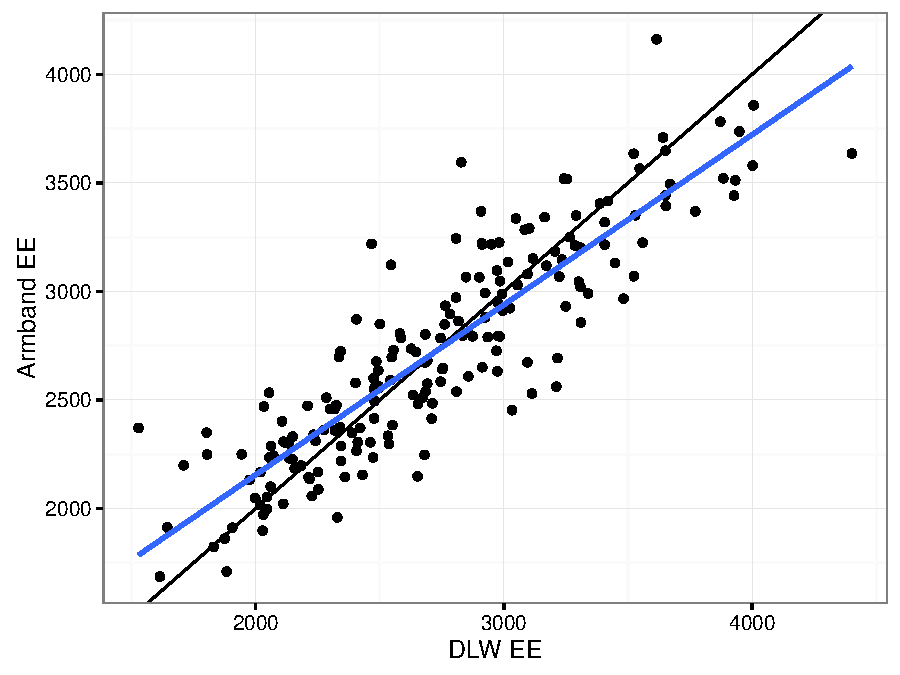
\includegraphics[width=.8\linewidth]{figure/armbandvsdlw-1} 

}



\end{knitrout}
\end{frame}

%-------------------


%---------------
\begin{frame}
\frametitle{Modeling Energy Balance}

\end{frame}
%--------------

\begin{frame}
\frametitle{Measurement Methods}

Measurement of EE and $\Delta$ES is less noisy than EI and true gold standard measurements exist

\begin{itemize}
\begin{multicols}{2}
\item Pedometer
\item Consumer grade wearables
\item Sensewear Armband
\item DLW (gold standard)

\columnbreak
\item Body Weight
\item Calipers
\item BodPod
\item Bioelectrical impedence
\item DXA (gold standard)
\end{multicols}
\end{itemize}

Notice how none of these methods require self report? 

\end{frame}

%-----------------


\section{Measurement Error Models}
\subsection{Statistical Model}

%-------------
\begin{frame}
\frametitle{Research Goal}

\begin{block}{Research Outcomes}
Our overall goal is to provide a cheap, easy, noninvasive \emph{prediction of EI for an individual in free living situations}
\end{block}

To achieve our goal:

\begin{itemize}
\item
Statistically assess the measurement error in various instruments of both EE and $\Delta$ES
\item 
Calibrate cheaper measures so they provide reasonable accuracy without the expense and expertise required for DLW and DXA
\end{itemize}

\end{frame}

%--------------
\begin{frame}
\frametitle{Data Required}

Because we are assessing the measurement error in these instruments, we need replicate measures of all EE and $\Delta$ES measurements on an individual that accounts for all measurement error.

This is a little tricky...
\begin{itemize}
\item
%For both cheap measures of EE and DLW, we need two periods of time measuring EE on each individual
Replicates measurements of EE for an individual
\item
%For both cheap measures $\Delta$ES and DXA, we need to measure body composition at the beginning of exercise period and end of exercise period, doing this procedure twice for each individual
Replicate measurements of $\Delta$ES for an individual
\item
Demographic covariates for an individual
\end{itemize}

Luckily, we have a wealth of data from the Energy Balance Study to help propose a model and empirically check assumptions.

\end{frame}


\subsection{Model Specification}

\begin{frame}
We can further specify forms for each component:

\begin{align}
Y_{ij}^{EE} &= m_{ee}(X_i^{EE}) + \gamma_{ee}Z_i + \epsilon_{ij}^{EE} \\
Y_{ij}^{\Delta ES} &= m_{es}(X_i^{\Delta ES}) + \gamma_{es}Z_i + \epsilon_{ij}^{\Delta ES} \\
W_{ij}^{EE} &= X_i^{EE} + \nu_{ij}^{EE} \\
W_{ij}^{\Delta ES} &= X_i^{\Delta ES} + \nu_{ij}^{\Delta ES}
\end{align}

\end{frame}

%--------------------%
\begin{frame}
\begin{itemize}
\item
Because we never can observe $(X_i^{EE},X_i^{\Delta ES})$, it is difficult to say the functional relationship ($m_{ee}$ and $m_{es}$) between it and cheap measurements $Y^{EE}$ and $Y^{\Delta ES}$ 

\item
Because of this, we choose to model $m_{ee}$ and $m_{es}$ with B-splines
\item
Must specify number of knots $k$ and knot locations $\zeta_1,...\zeta_k$
\end{itemize}

\begin{align}
m_{ee}(X_i^{EE}) &= \sum_{i=1}^{k_{ee}} b_{i,ee}(\zeta_{i,ee}) \beta_{i,ee} = B_{ee}(\zeta_{ee}) \beta_{i,ee} \\
m_{es}(X_i^{\Delta ES}) &= \sum_{i=1}^{k_{es}} b_{i,es}(\zeta_{i,es}) \beta_{i,es} = B_{es}(\zeta_{es}) \beta_{i,es}
\end{align}

We let $k$ and $\zeta_1,...\zeta_k$ vary according to the data

\end{frame}

%--------------
\begin{frame}
\frametitle{Specifying the Likelihood}

%%%%%%%%%%%%%%%%%%%%%%%%%%%%%%%%%
%%%%%%%%%%%%%%%%%%%%%%%%%%%%%%%%%%
%get two column
\begin{align}
\epsilon_{ij}^{EE} &\overset{iid}{\sim} N(0,\sigma_{i,yee}^2) \\
\epsilon_{ij}^{\Delta ES} &\overset{iid}{\sim} N(0,\sigma_{i,yes}^2) \\
\nu_{ij}^{EE} &\overset{iid}{\sim} N(0,\sigma_{i,wee}^2) \\
\nu_{ij}^{\Delta ES} &\overset{iid}{\sim} N(0,\sigma_{i,wes}^2) 
\end{align}

\end{frame}

%-------------
\begin{frame}
\frametitle{Latent Variable Likelihood}

The final component to have a joint likelihood specified is the bivariate latent variable. Because we \emph{never ever} observe these values, we must specify its distribution carefully

\begin{align}
(X_i^{EE}, X_i^{\Delta ES}) &\overset{iid}{\sim} \sum_{h=1}^{\infty} \pi_h N(\mu_h,\Sigma_h) \\
\pi_h &\overset{iid}{\sim} Stick(\alpha) \\
 & \sum_{h=1}^{\infty} \pi_h = 1 \\
 \pi_h &= V_h \prod_{\ell <  h} (1-V_h) \\
 V_H &= 1\\
 V_h &\sim Beta(1,\alpha), h<H
\end{align}

\end{frame}

%-------------
\begin{frame}
\frametitle{Priors}
Need to assign priors for unknown parameters 
\begin{align}
\boldsymbol{\theta} &= (\{\sigma_{i,yee} \}_{i=1}^{n}, \{\sigma_{i,yes}\}_{i=1}^{n} , \{\sigma_{i,wee}\}_{i=1}^{n} , \\
& \{\sigma_{i,wes}\}_{i=1}^{n} ,\{\Sigma_{i}\}_{i=1}^{n} , \{\gamma_{i,yee}\}_{i=1}^{p} , \\
& \{\gamma_{i,yes}\}_{i=1}^{p} , \{\beta_{i,yee}\}_{i=1}^{k_{ee}} , \{\beta_{i,yes}\}_{i=1}^{k_{kes}}, k_{ee}, k_{es}, \\
& \{\zeta_{i,ee} \}_{i=1}^{k_{ee}},\{\zeta_{i,es} \}_{i=1}^{k_{es}})
\end{align}

\end{frame}

%------------------
\begin{frame}
Assume independent priors (for now)

\begin{multicols}{2}
\begin{align}
p(\sigma_{i,yee}) \overset{iid}{\sim} C^+(0,1) \\
p(\sigma_{i,yes}) \overset{iid}{\sim} C^+(0,1) \\
p(\sigma_{i,wee}) \overset{iid}{\sim} C^+(0,1) \\
p(\sigma_{i,wes}) \overset{iid}{\sim} C^+(0,1) \\
p(\Sigma_i) \overset{iid}{\sim} \text{ Inv-Wish}(I_{2x2},3) 
\end{align}
\columnbreak
\begin{align}
p(\gamma_{i,ee}) &\overset{iid}{\sim} N(w_{i,ee},B_{i,ee}) \\
p(\gamma_{i,es}) &\overset{iid}{\sim} N(w_{i,es},B_{i,es}) \\
p(\beta_{i,ee}) &\overset{iid}{\sim} N(v_{i,ee},C_{i,ee}) \\
p(\beta_{i,es}) &\overset{iid}{\sim} N(v_{i,es},C_{i,es}) \\
p(k_{ee}) &{\sim} Poi(a_{ee}) \\
p(k_{es}) &{\sim} Poi(a_{es}) 
\end{align}
\end{multicols}
\begin{align}
p(\zeta_1,...,\zeta_{k_{ee}}|k_{ee}) &\sim DUnif(x_1^{EE},...,x_n^{EE}) \\
p(\zeta_1,...,\zeta_{k_{es}}|k_{es}) &\sim DUnif(x_1^{\Delta ES},...,x_n^{\Delta ES})
\end{align}

Priors likely to change as we elicit expert information and use of past data

\end{frame}

\subsection{Estimation}

%---------------
\begin{frame}
\frametitle{Estimation}
Since we are taking a Bayesian approach, the posterior distribution $p(\boldsymbol{\theta}|Y,W,Z)$ gives us everything we need for inference

\begin{itemize}
\item
Using Bayes Rule: 
\begin{align}
p(\boldsymbol{\theta}|Y,W,Z) &= \frac{p(Y,W|\boldsymbol{\theta},Z) p(\boldsymbol{\theta})}{\int p(Y,W,\boldsymbol{\theta}|Z) d\boldsymbol{\theta}}
\end{align}
\item 
Integral is impossible to evaluate analytically, use MCMC to simulate draws from joint posterior
\item
Will use Gibbs Sampler to update parameters 
\item
Reversible Jump MCMC step necessary for B-splines since number of knots $k$ and knot locations $\zeta_1,...\zeta_k$ are random variables and therefore dimension of posterior is allowed to change
\item
Implement in R/C++
\end{itemize}

\end{frame}

%-------------
\subsection{Model Assessment and Inference}

%-------------
\begin{frame}
\frametitle{Model Assessment and Comparason}
We will assess the fit of our model through the use of the posterior predictive distributions and relevant discrepancy measures $D()$

\begin{align}
  \label{ypostpred}
  p(Y^*|W,Y,Z) &= \int \int p(Y^*|\boldsymbol{\theta},X,Z) p(\boldsymbol{\theta}, X|Y,W) d\boldsymbol{\theta} dX \\
  \label{wpostpred}
  p(W^*|W,Y,Z) &= \int \int p(W^*|\boldsymbol{\theta},X,Z) p(\boldsymbol{\theta}, X|Y,W) d\boldsymbol{\theta} dX \\
  \label{xpostpred}
  p(X^*|W,Y,Z) &= \int \int p(X^*|\boldsymbol{\theta}) p(\boldsymbol{\theta}, X|Y,W) d\boldsymbol{\theta} dX
\end{align}

For each simulated replicate data set (for each $Y,W,X$) calculate $D()$. Compare to $D()$ from true data

\end{frame}

%----------------
\begin{frame}
\frametitle{Model Comparason}
Although I presented only one specific model here, there are simplifying (and more complicating) assumptions we could (and will) make. To compare models we can use:

\begin{itemize}
\item
DIC
\item 
Bayes Factors
\item
PMSE of EI --- this is not straightforward
\item
Parsimony and Practical Interpretation
\end{itemize}

\end{frame}

%----------------




\end{document}

